% small.tex
\documentclass[12pt]{beamer}
\usetheme{amcg}
\beamertemplatenavigationsymbolsempty
\renewcommand{\thefootnote}{}
\providecommand{\e}[1]{\ensuremath{\times 10^{#1}}}
\usepackage{mathptmx}
\usepackage{helvet}
\usepackage{color}
\newcommand\TILDE{\char`\~}
\usepackage{listings}

% items enclosed in square brackets are optional; explanation below
\title[Fluidity]{Obtaining and Compiling Fluidity}
\subtitle[]{}
\institute{1 - Dept of Earth Science and Engineering, Imperial College London}
\author[Tim Greaves]{\large{Tim Greaves}\inst{1}}
\date{}


\begin{document}


%--- the titlepage frame -------------------------%
\begin{frame}
  \titlepage
\end{frame}

\begin{frame}
  \frametitle{Session Overview}
\begin{itemize}
    \item Installing Fluidity from packages
    \item Obtaining Fluidity sourcecode
    \item GitHub and Buildbot
    \item Configuring, building, testing and installing
    \item A brief introduction to running Fluidity
    \item Updating Fluidity
\end{itemize}
\end{frame}


\section{Getting Fluidity}
\begin{frame}
        \frametitle{How to obtain Fluidity}
\begin{itemize}
    \item {\bf Binary} (release only)
	  \\Prebuilt packages are available for Ubuntu LTS, Red Hat 6 (and
              derivatives), and OpenSuSE (not officially supported)
    \item {\bf Source} (release, trunk or branch)
	  \\Available from GitHub as a tarball (release only) or git repository
\end{itemize}
\end{frame}

\begin{frame}[fragile]
        \frametitle{Installing the Fluidity package: Ubuntu}
\lstset{language=bash}
Add the Fluidity package repository to your system:
\begin{lstlisting}[language=bash,basicstyle=\ttfamily\scriptsize]
sudo apt-add-repository -y ppa:fluidity-core/ppa
sudo apt-get update
\end{lstlisting}
Then install Fluidity:
\begin{lstlisting}[language=bash,basicstyle=\ttfamily\scriptsize]
sudo apt-get -y install fluidity
\end{lstlisting}
This is a ready-to-run binary package and comes with a PDF manual and the
Fluidity examples.
\end{frame}

\begin{frame}[fragile]
        \frametitle{Installing the Fluidity package: Red Hat}
\lstset{language=bash}
RHEL (Or CentOS) 6.5 is recommended for Fluidity, and requires the EPEL
repository to be enabled 

\hspace{10mm}(see http://fedoraproject.org/wiki/EPEL). 

Add the Fluidity repository to your system:
\begin{lstlisting}[language=bash,basicstyle=\ttfamily\scriptsize]
sudo yum-config-manager --add-repo \
  https://fluidityproject.github.com/yum/fluidity-rhel6.repo
\end{lstlisting}
Then install Fluidity:
\begin{lstlisting}[language=bash,basicstyle=\ttfamily\scriptsize]
sudo yum install fluidity
\end{lstlisting}
This is a ready-to-run binary package and comes with a PDF manual and the
Fluidity examples.
\end{frame}

\begin{frame}[fragile]
        \frametitle{Downloading Sourcecode}
\lstset{language=bash}
The source code for the latest release of Fluidity can be downloaded from:
\begin{lstlisting}[language=bash,basicstyle=\ttfamily\scriptsize]
https://github.com/FluidityProject/fluidity/releases/latest
\end{lstlisting}    
The latest development source for Fluidity (`master branch') can be cloned using git:
\begin{lstlisting}[language=bash,basicstyle=\ttfamily\scriptsize]
git clone https://github.com/FluidityProject/fluidity.git
\end{lstlisting}    
\end{frame}

\begin{frame}
        \frametitle{http://github.com/FluidityProject}
\begin{center}
    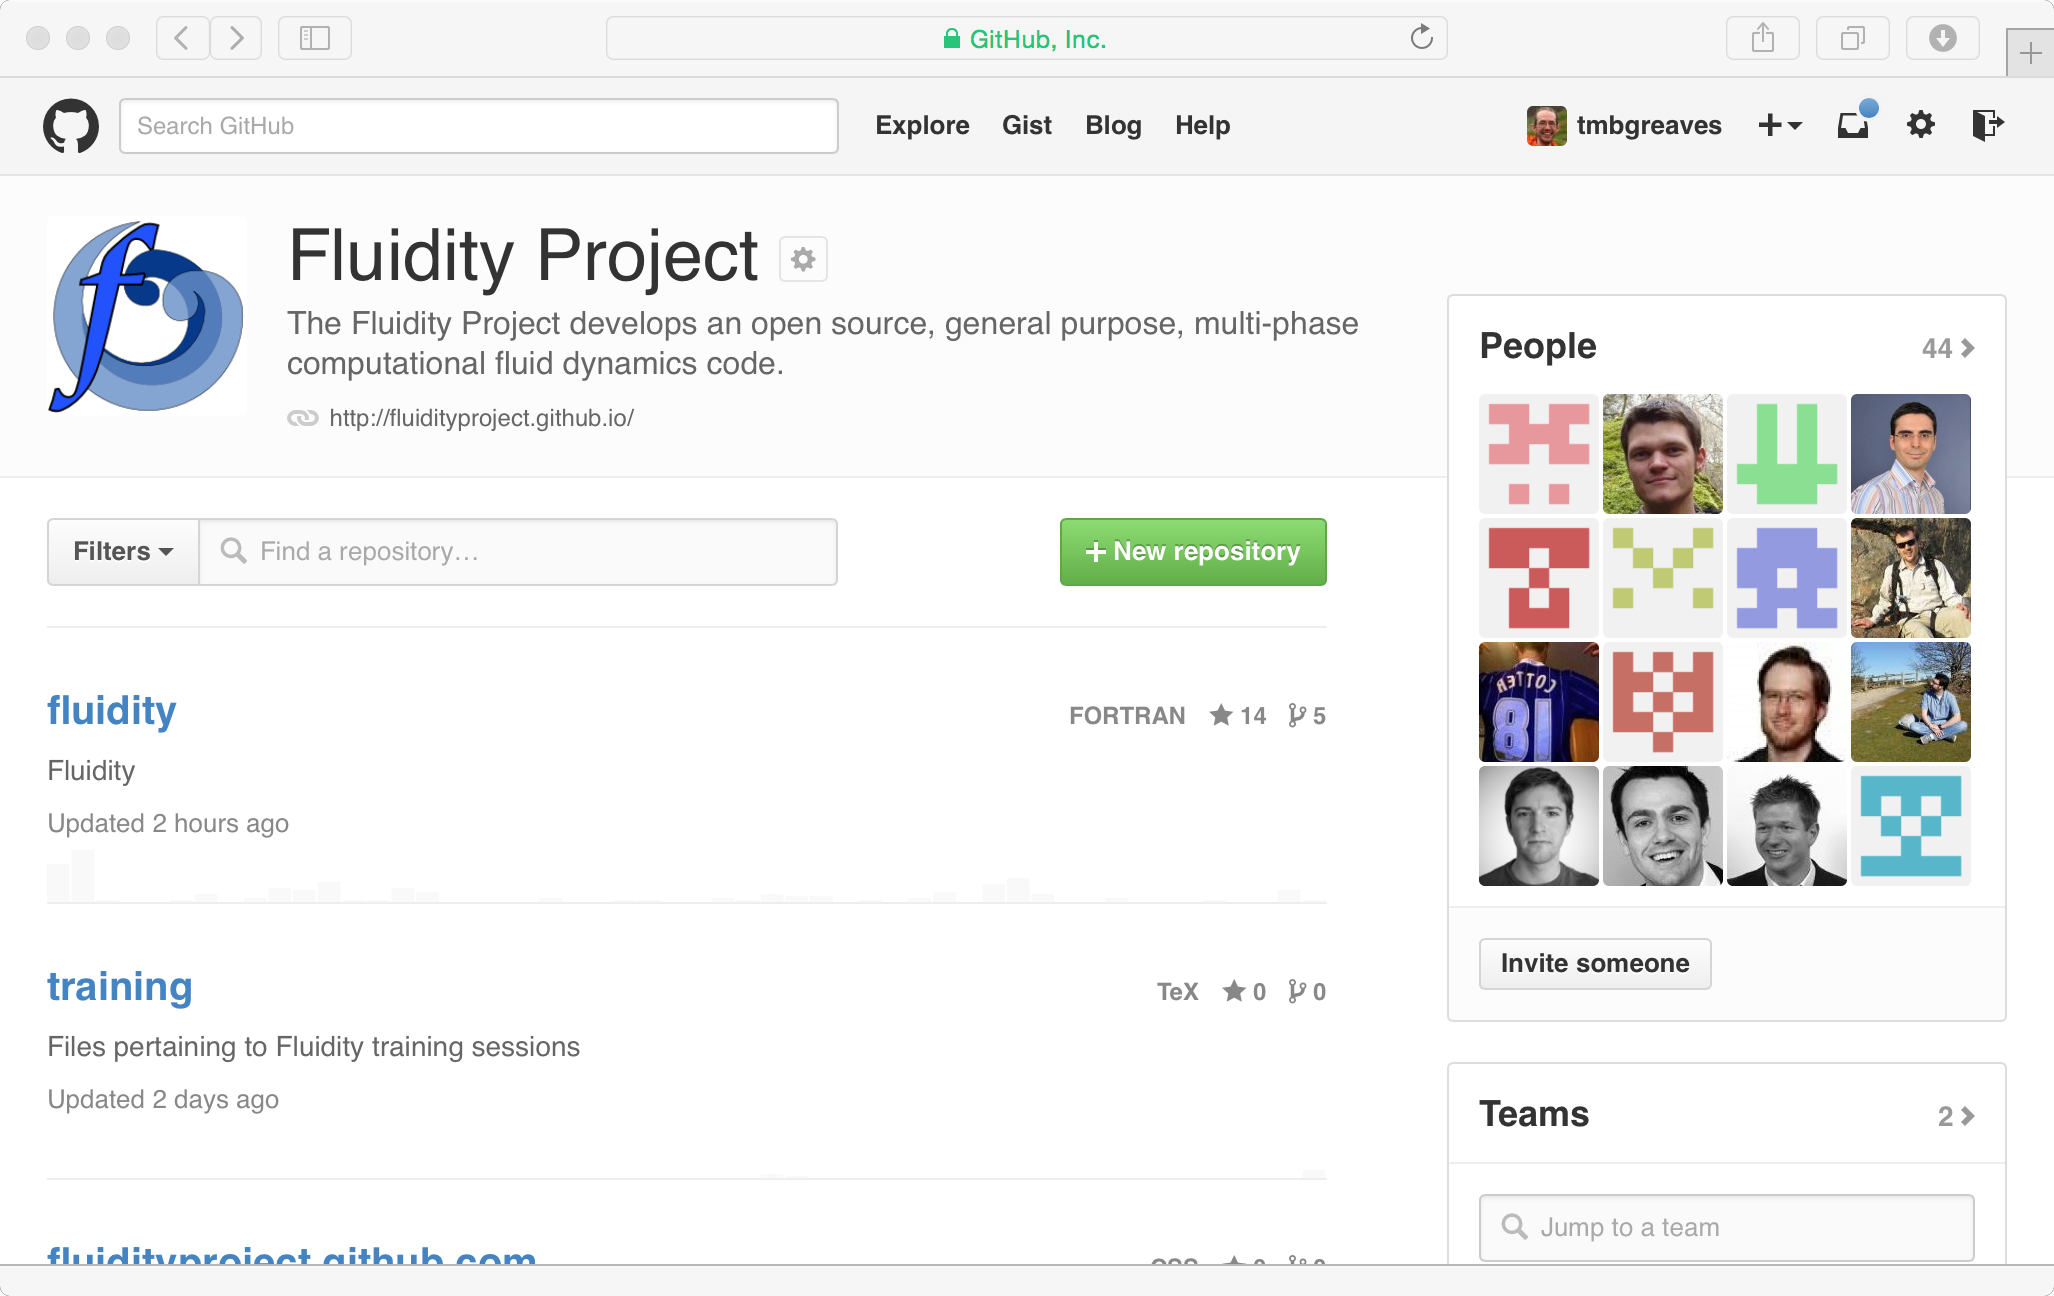
\includegraphics[width=0.9\textwidth]{images/github-home.png}
\end{center}
\end{frame}

\begin{frame}
        \frametitle{http://github.com/FluidityProject}
\begin{center}
    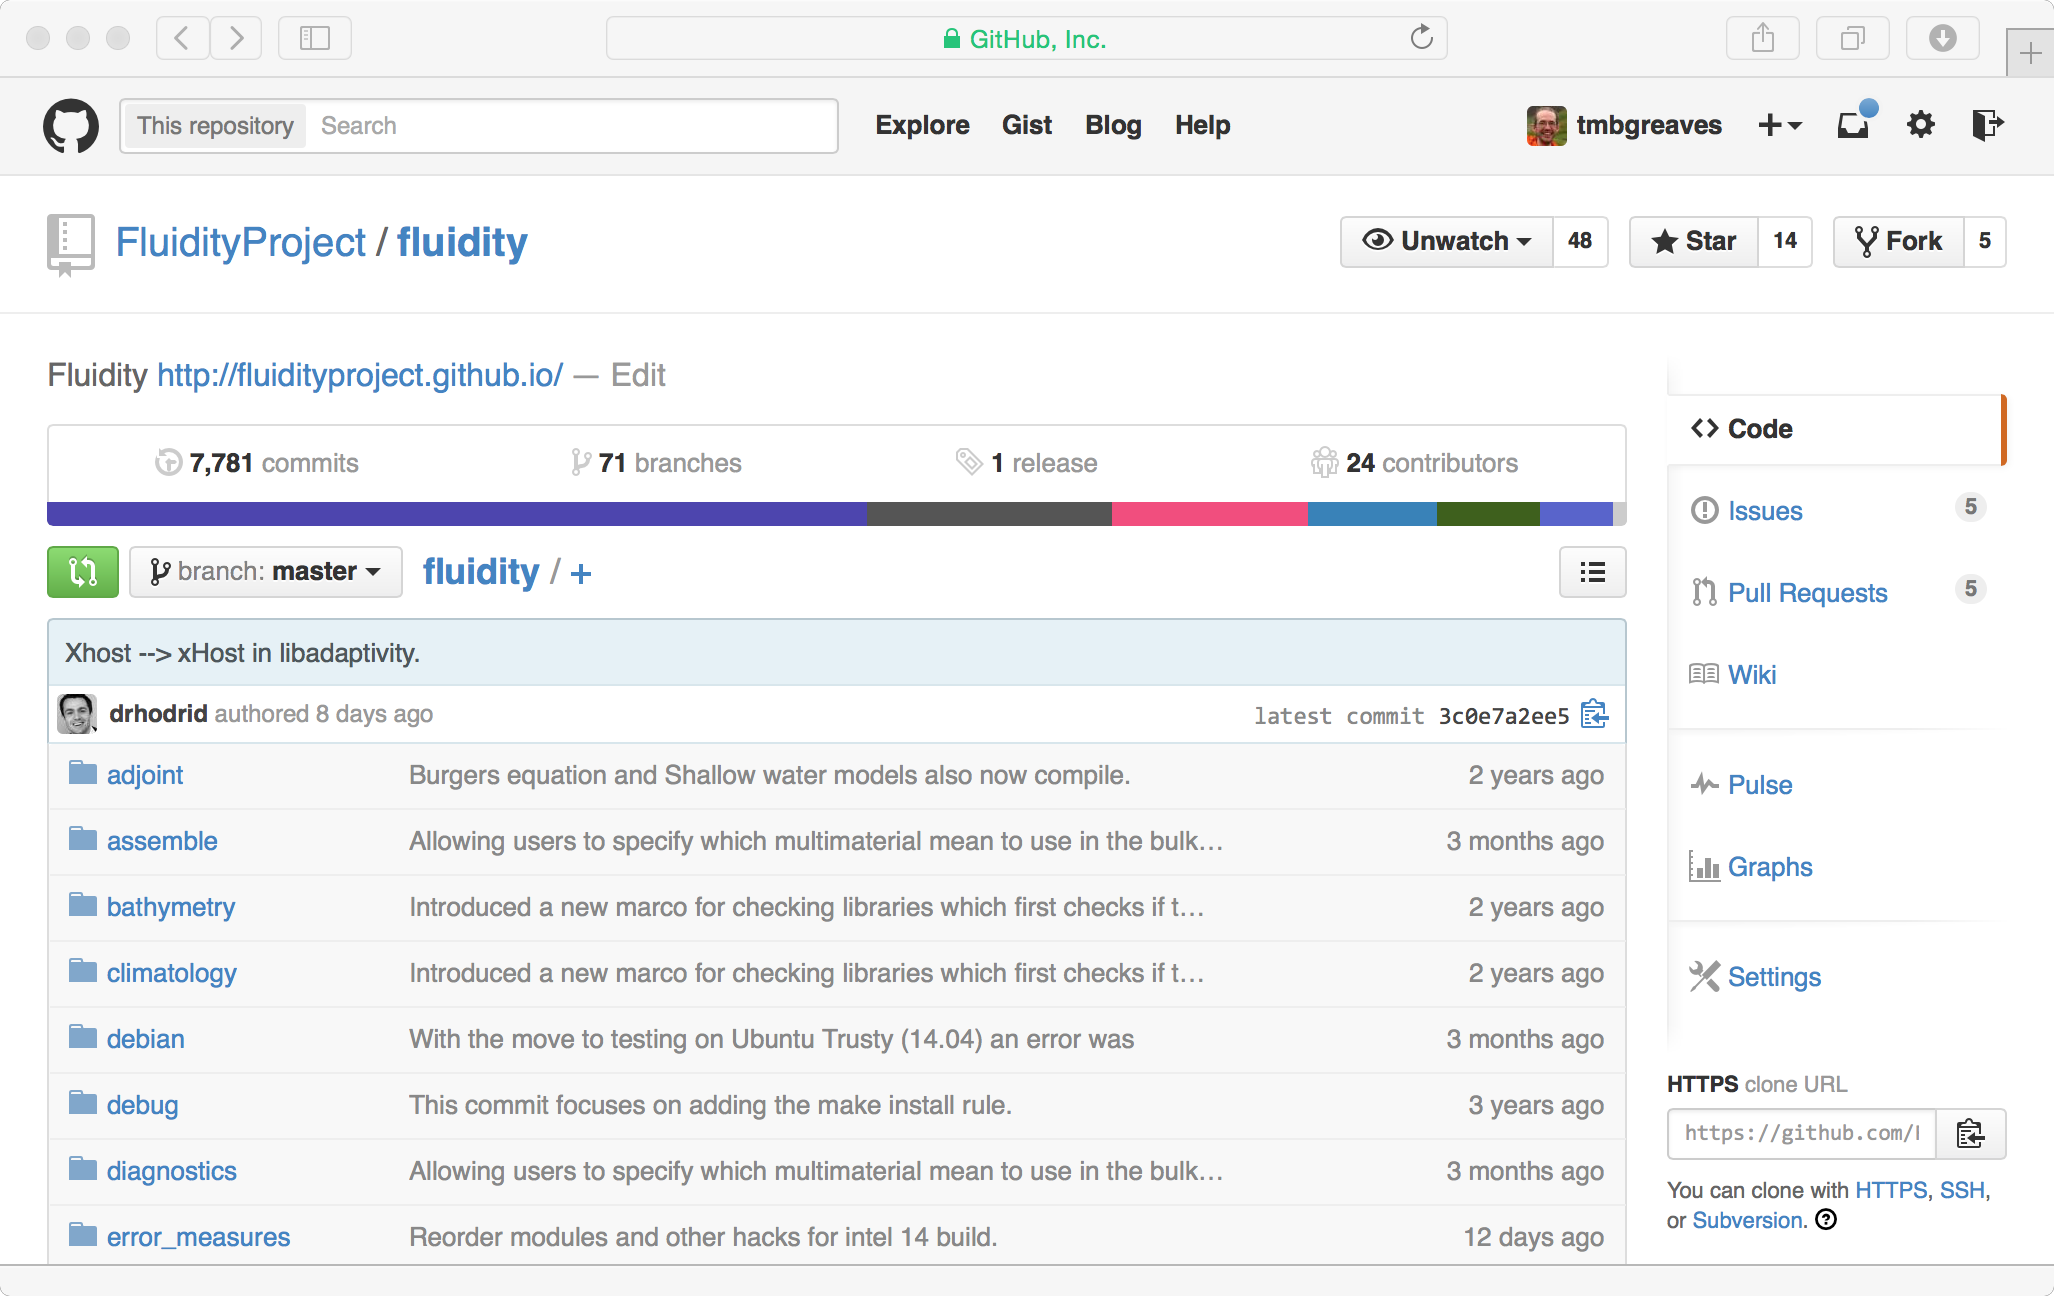
\includegraphics[width=0.9\textwidth]{images/github-master.png}
\end{center}
\end{frame}

\begin{frame}
        \frametitle{http://github.com/FluidityProject}
\begin{center}
    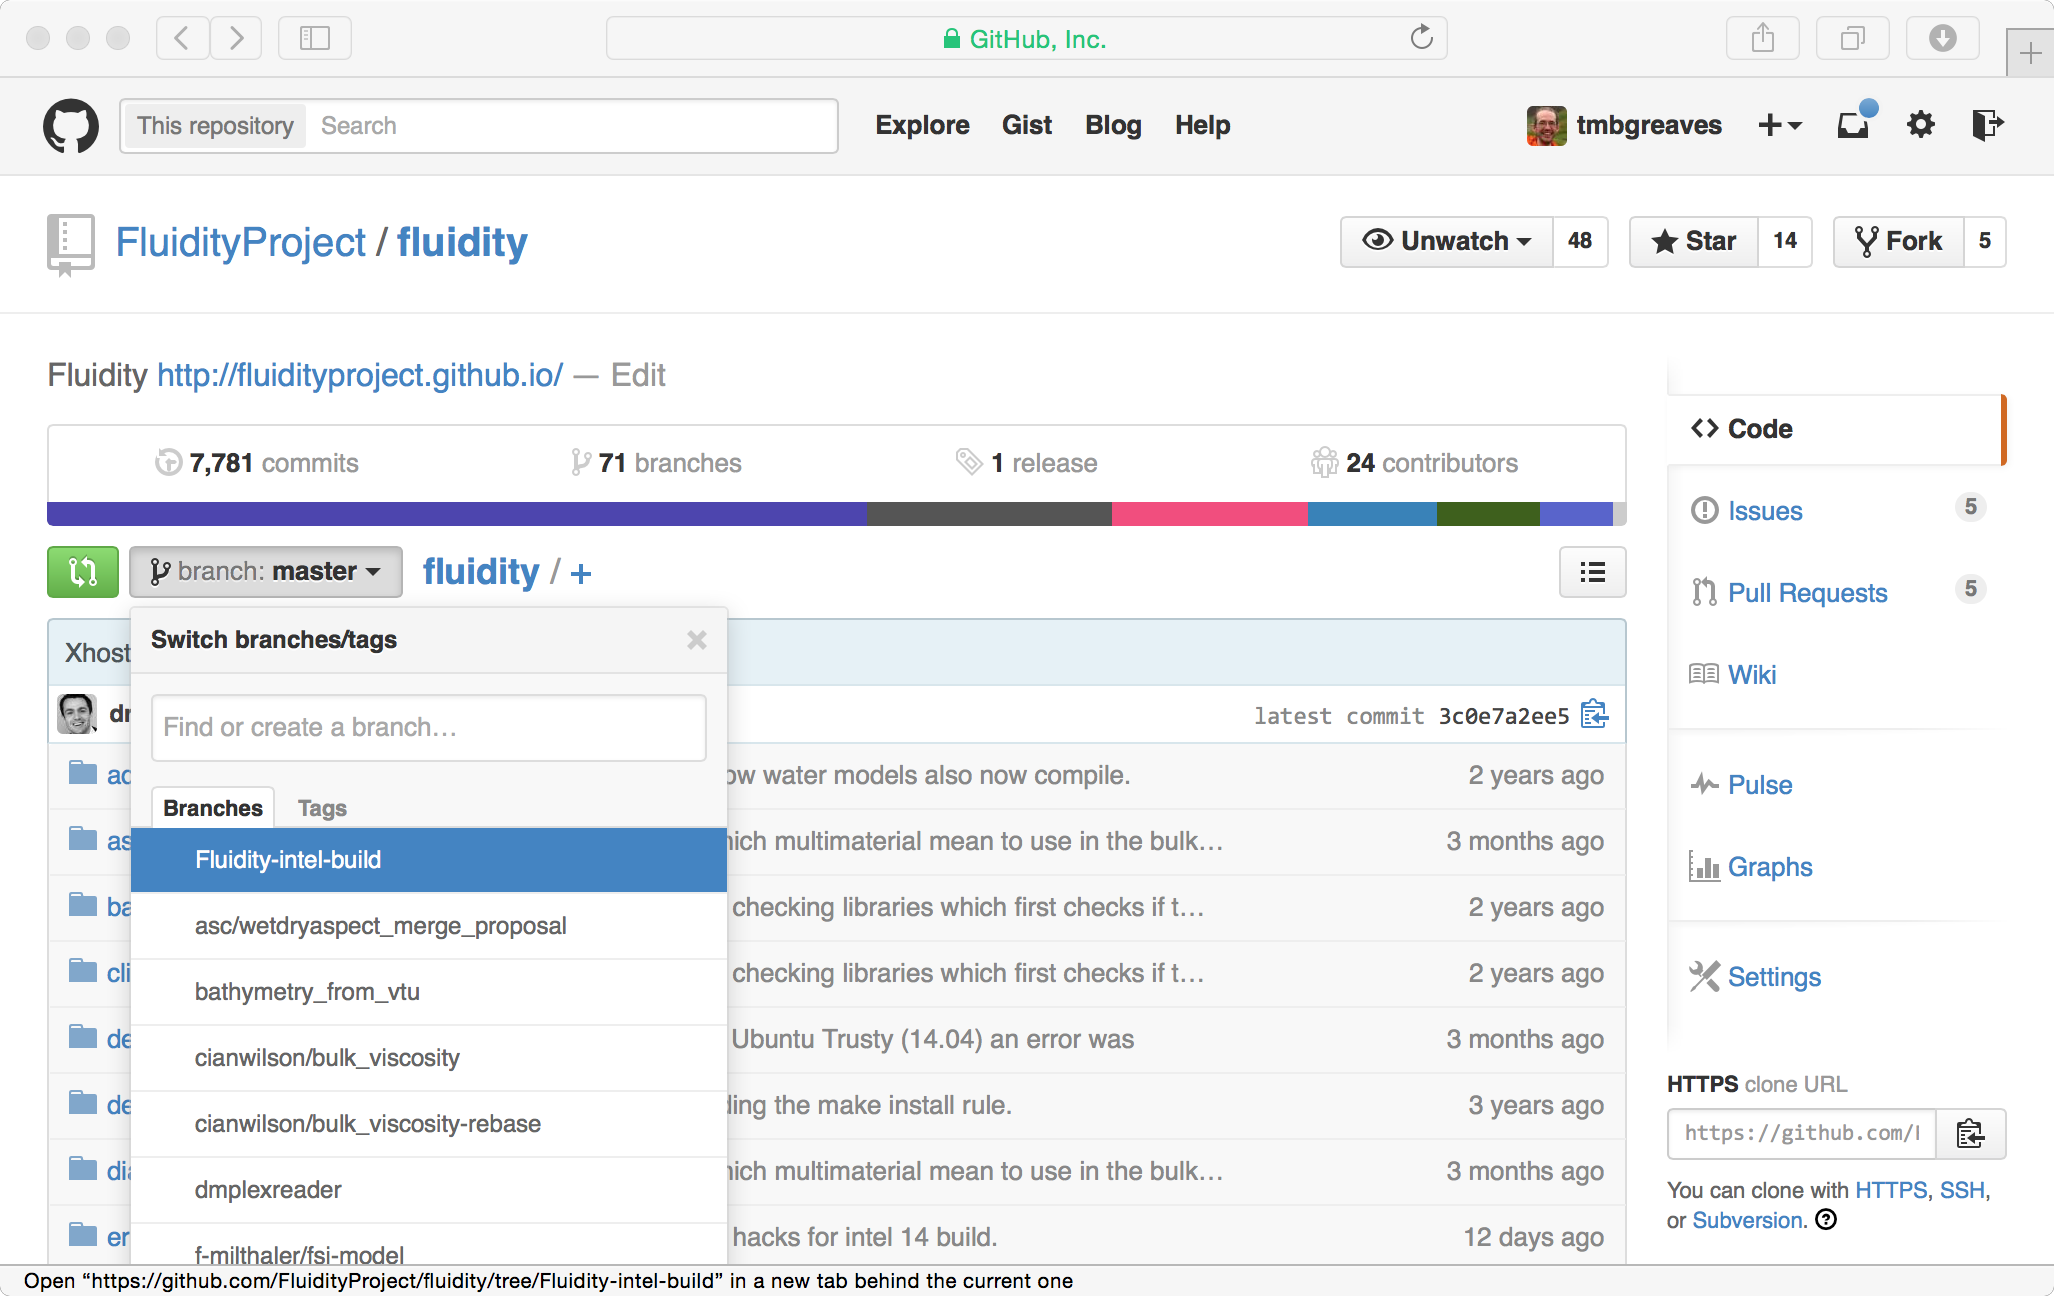
\includegraphics[width=0.9\textwidth]{images/github-changebranch.png}
\end{center}
\end{frame}

\begin{frame}
        \frametitle{http://github.com/FluidityProject}
\begin{center}
    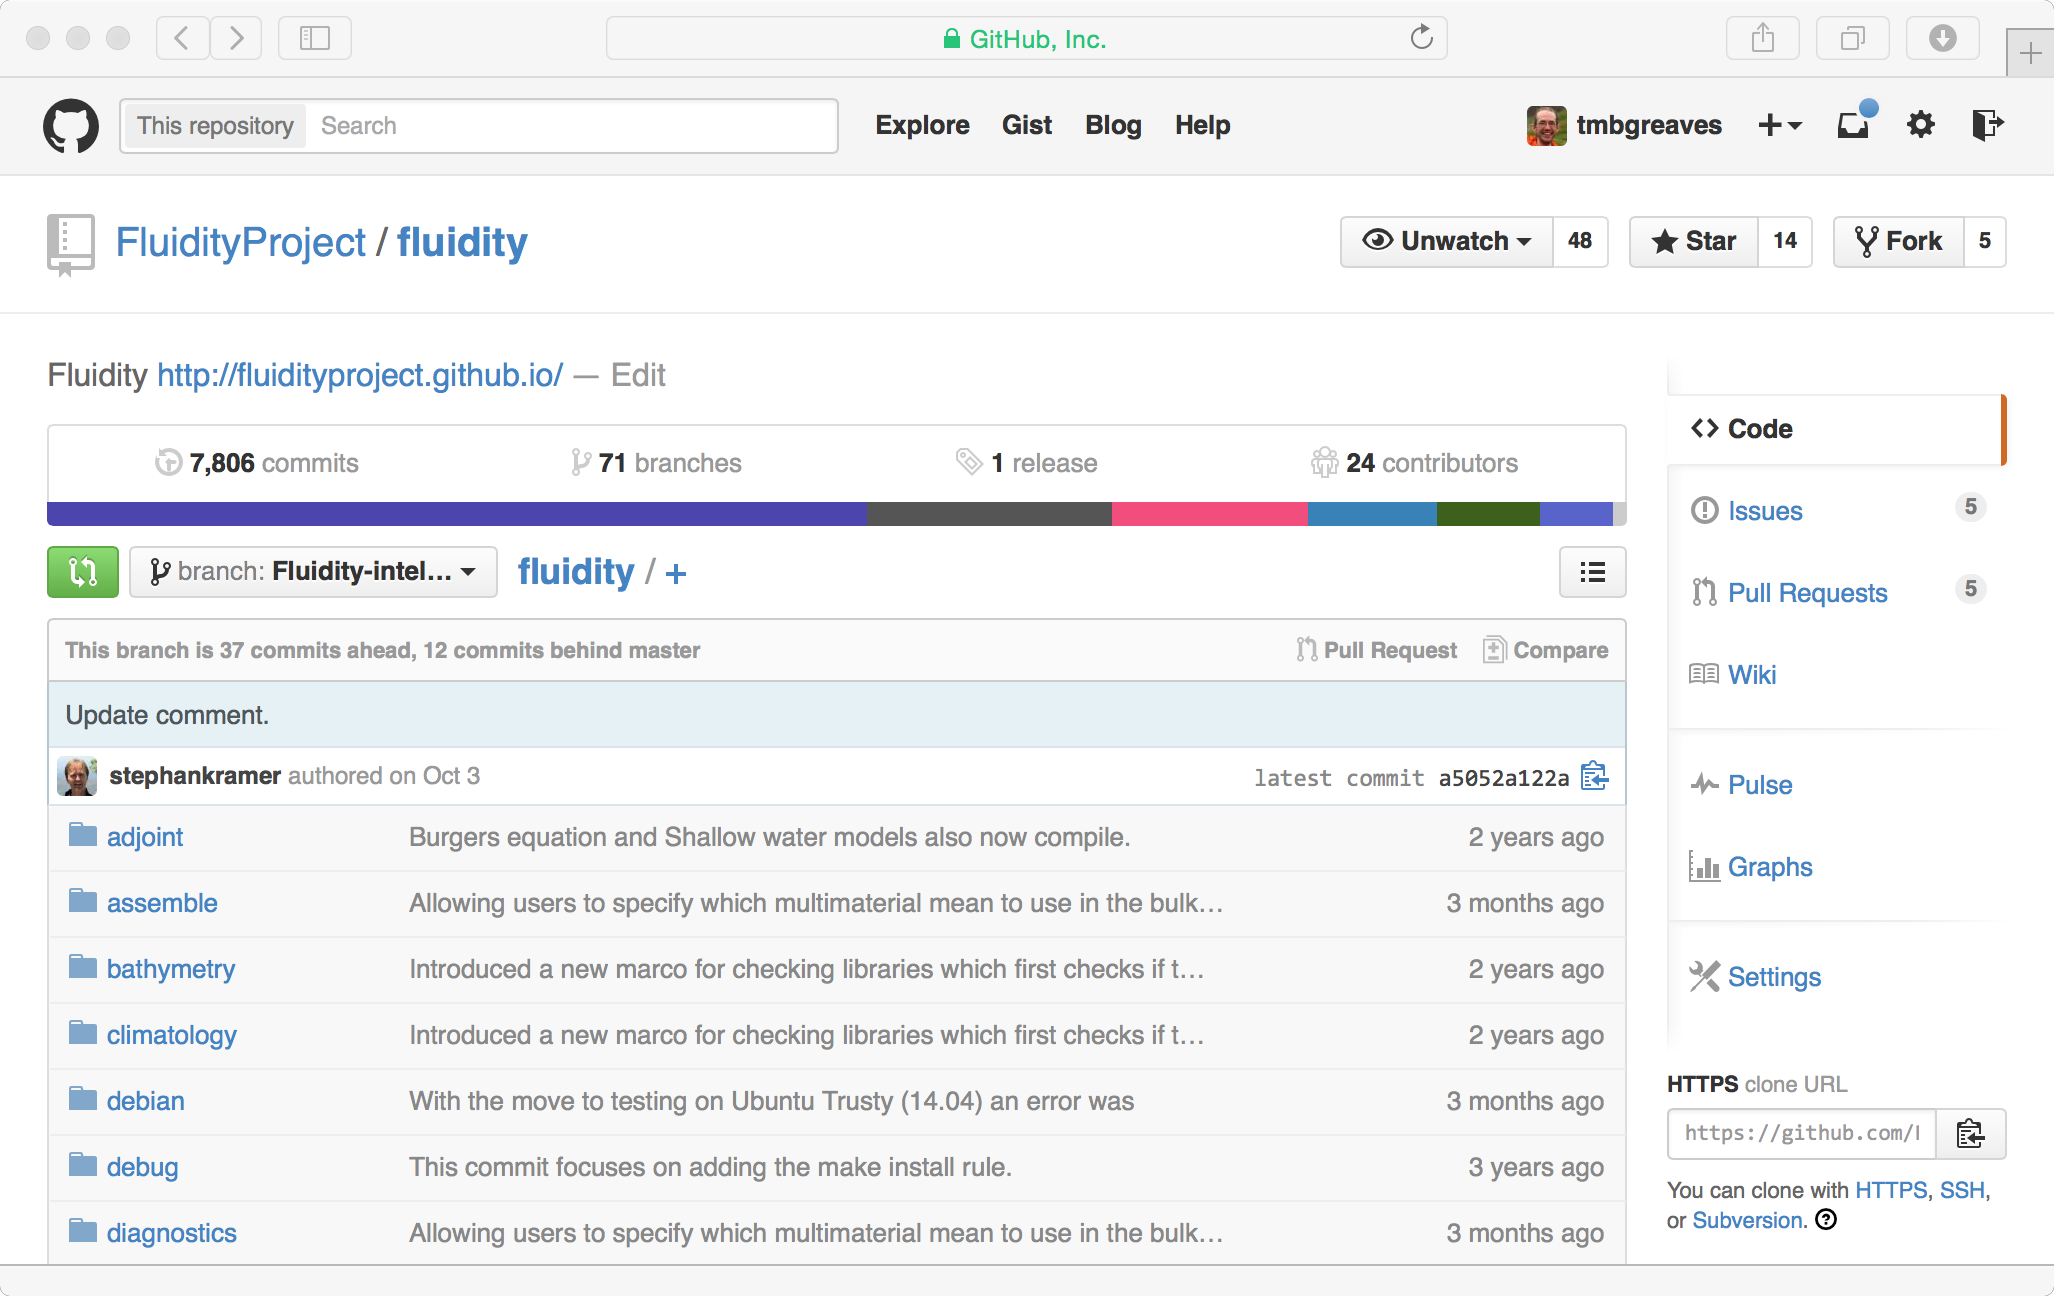
\includegraphics[width=0.9\textwidth]{images/github-changedbranch.png}
\end{center}
\end{frame}

\begin{frame}
        \frametitle{http://github.com/FluidityProject}
\begin{center}
    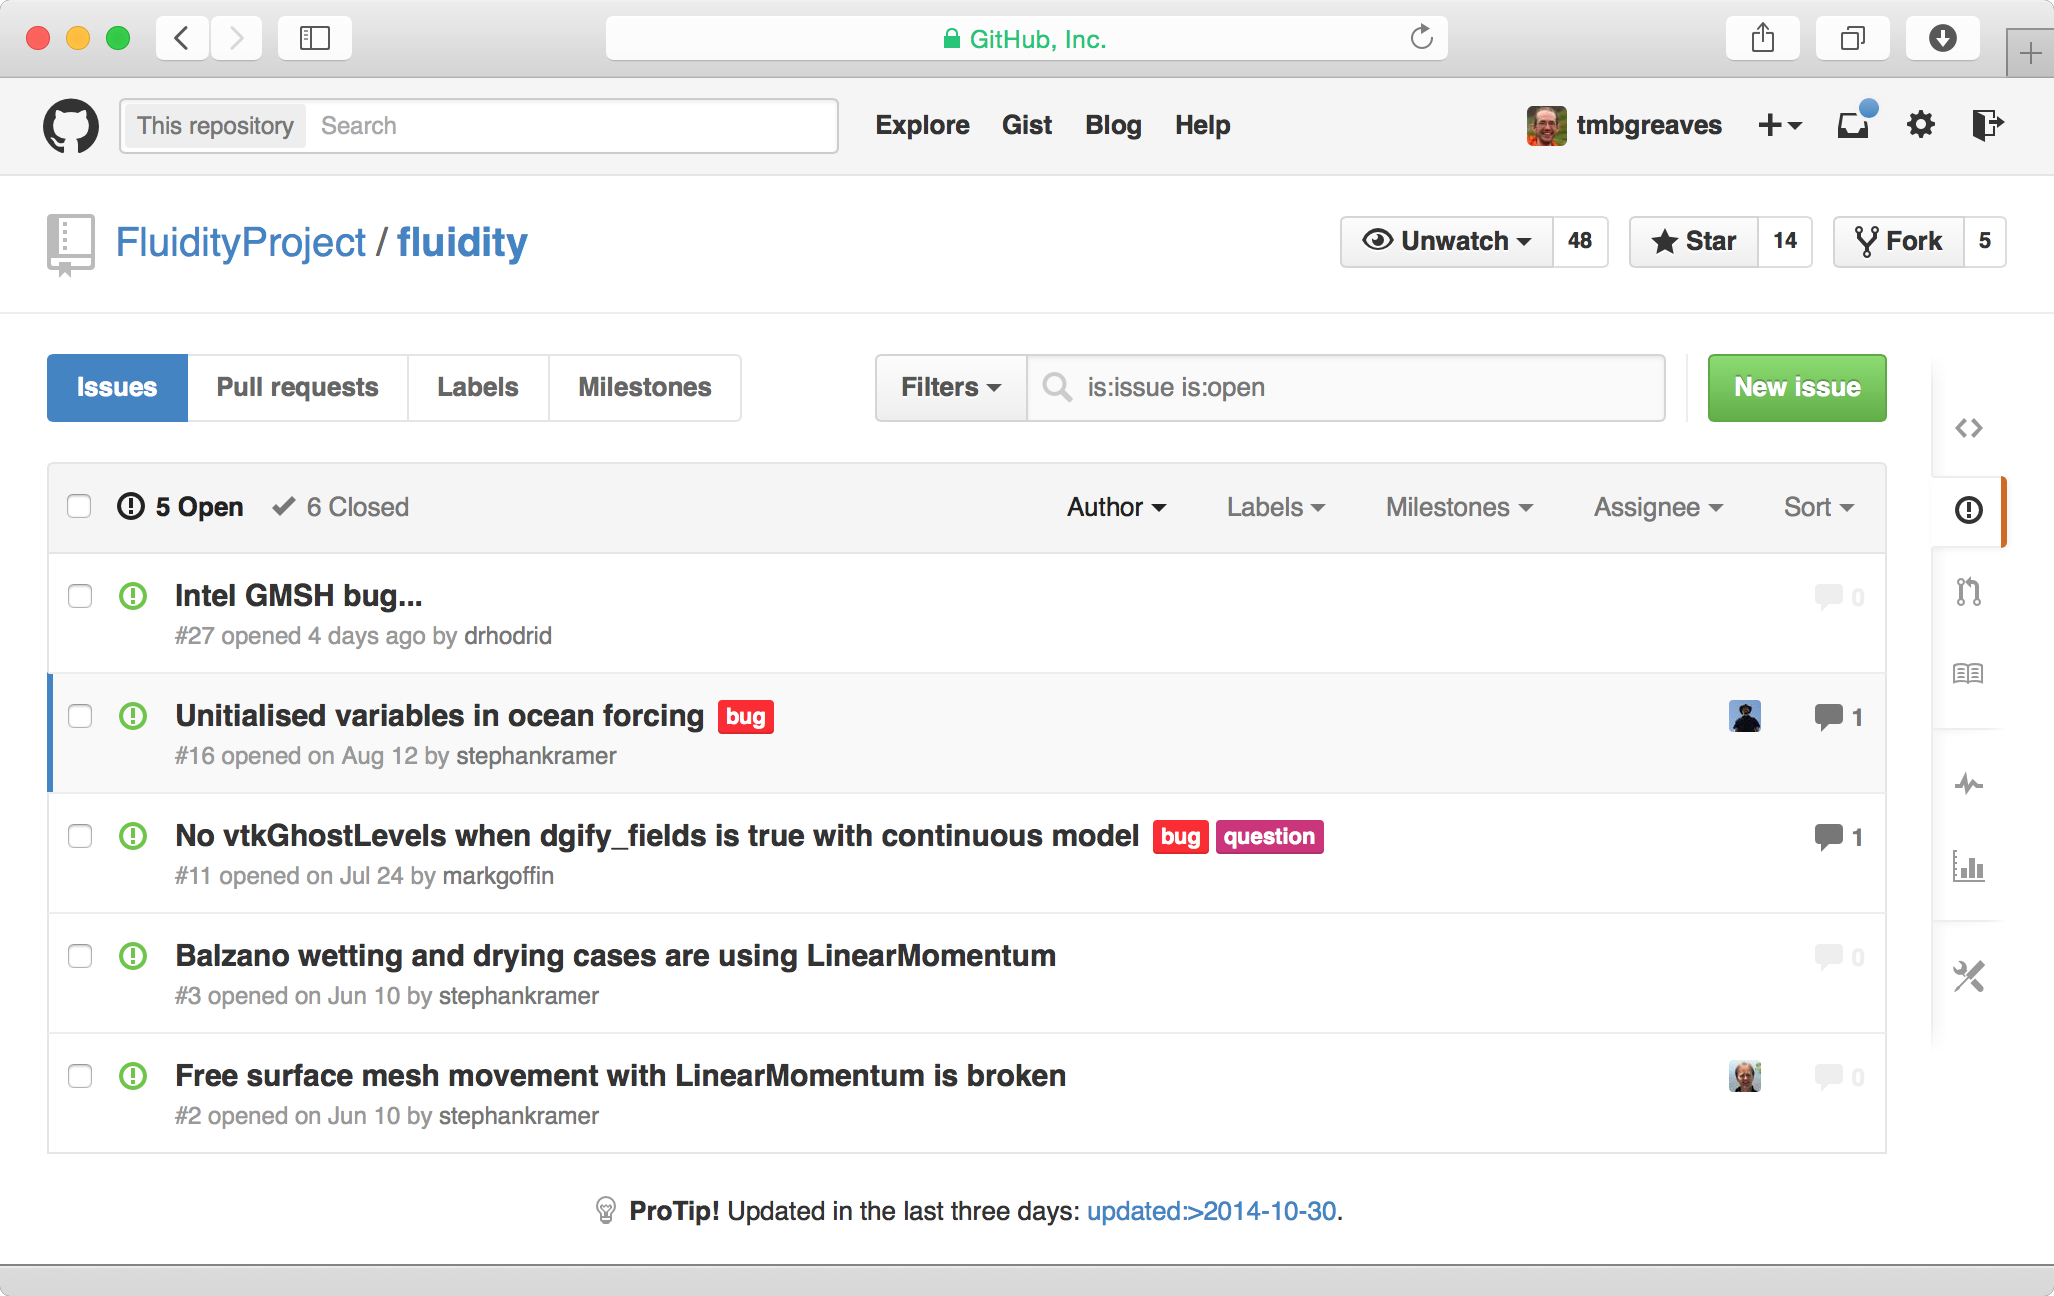
\includegraphics[width=0.9\textwidth]{images/github-issues.png}
\end{center}
\end{frame}

\begin{frame}
        \frametitle{http://github.com/FluidityProject}
\begin{center}
    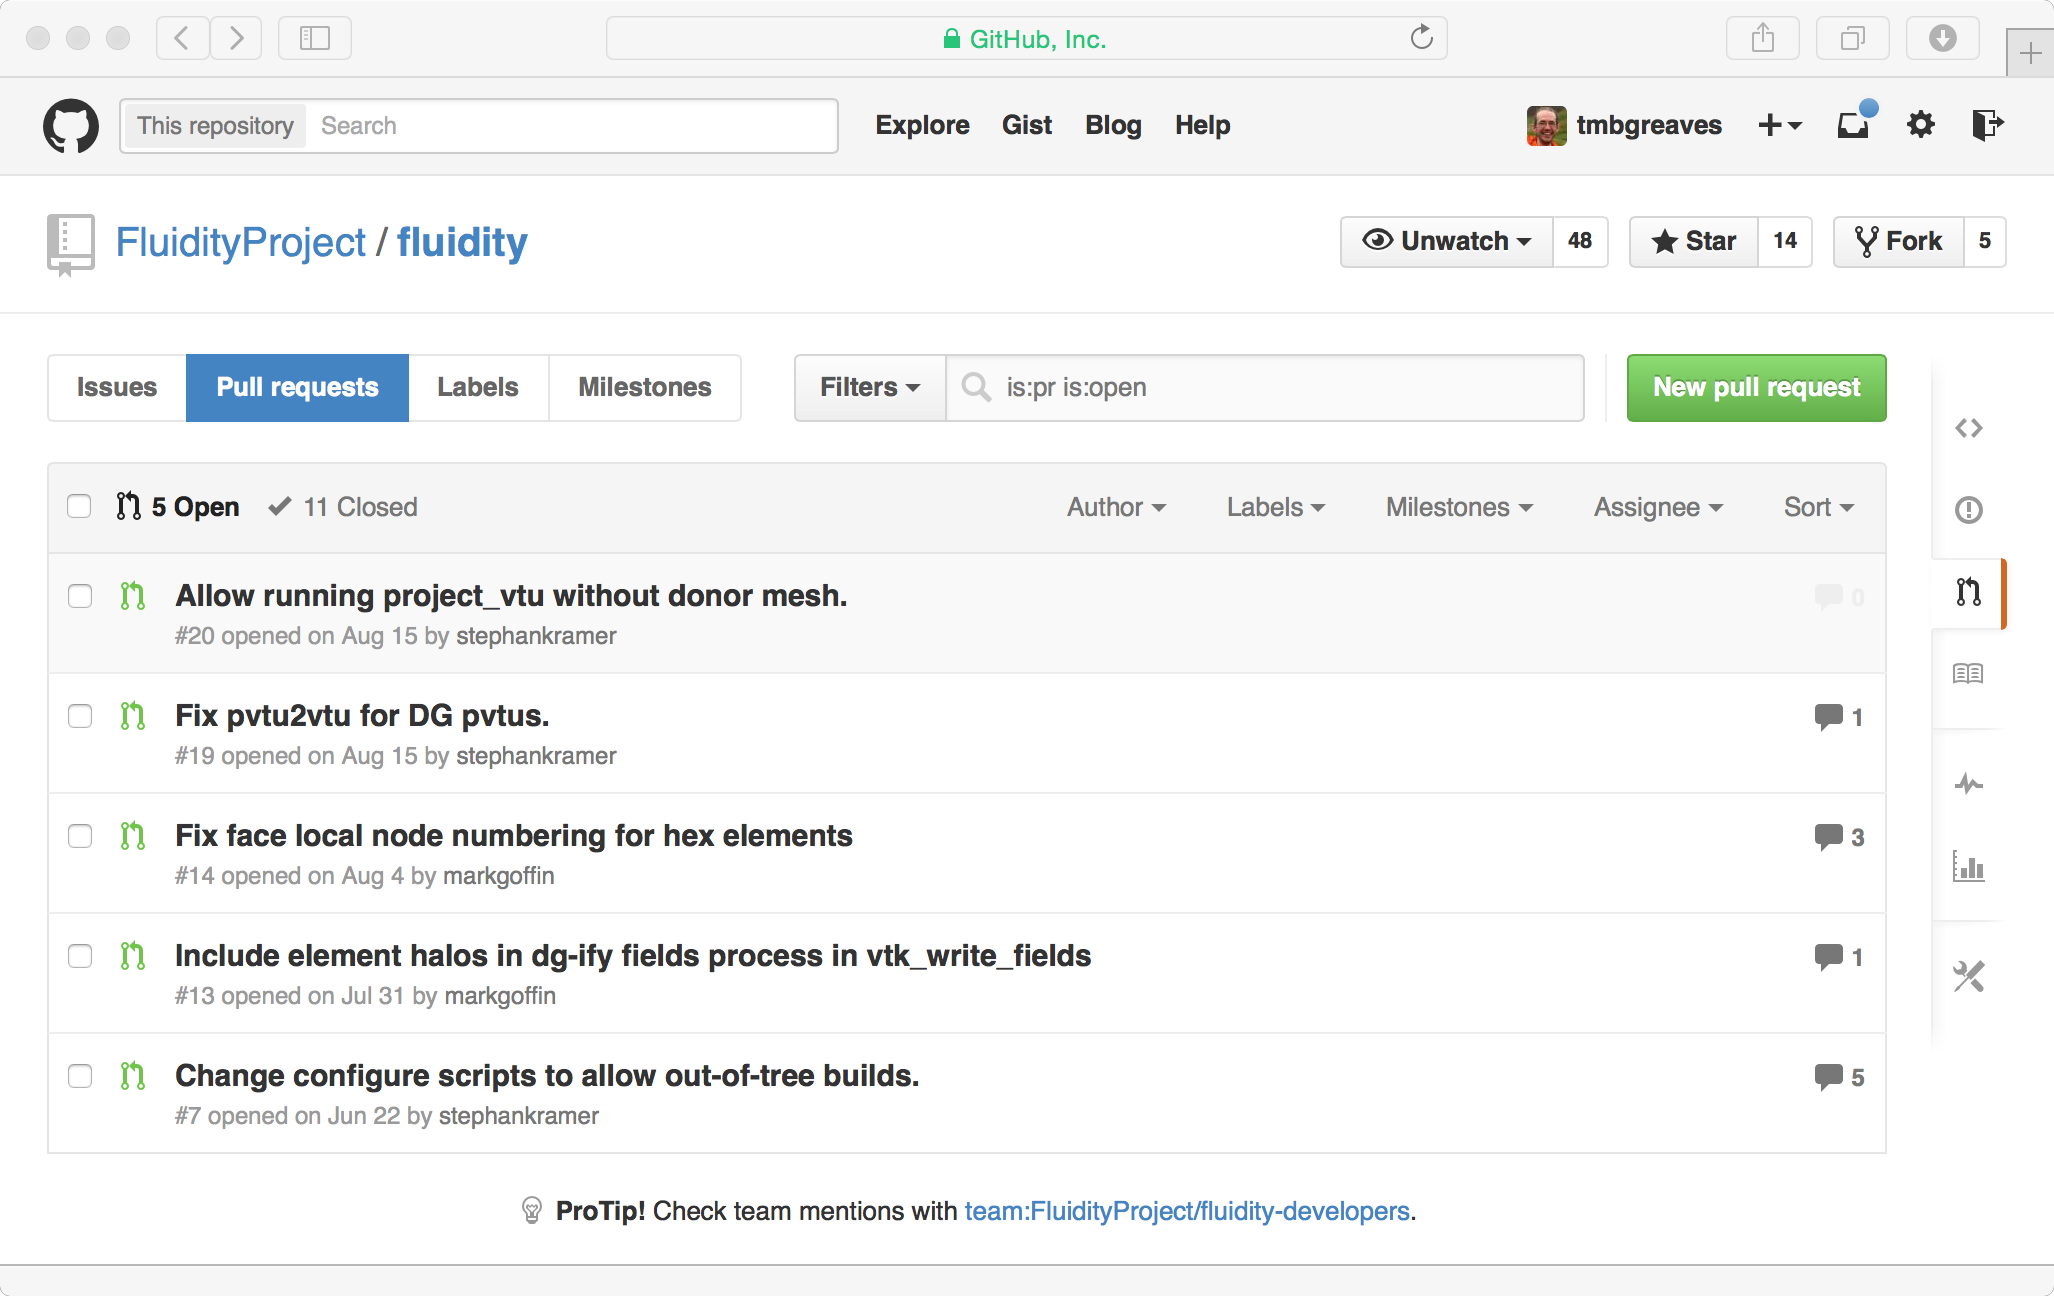
\includegraphics[width=0.9\textwidth]{images/github-pullrequests.png}
\end{center}
\end{frame}

\begin{frame}
        \frametitle{http://github.com/FluidityProject}
\begin{center}
    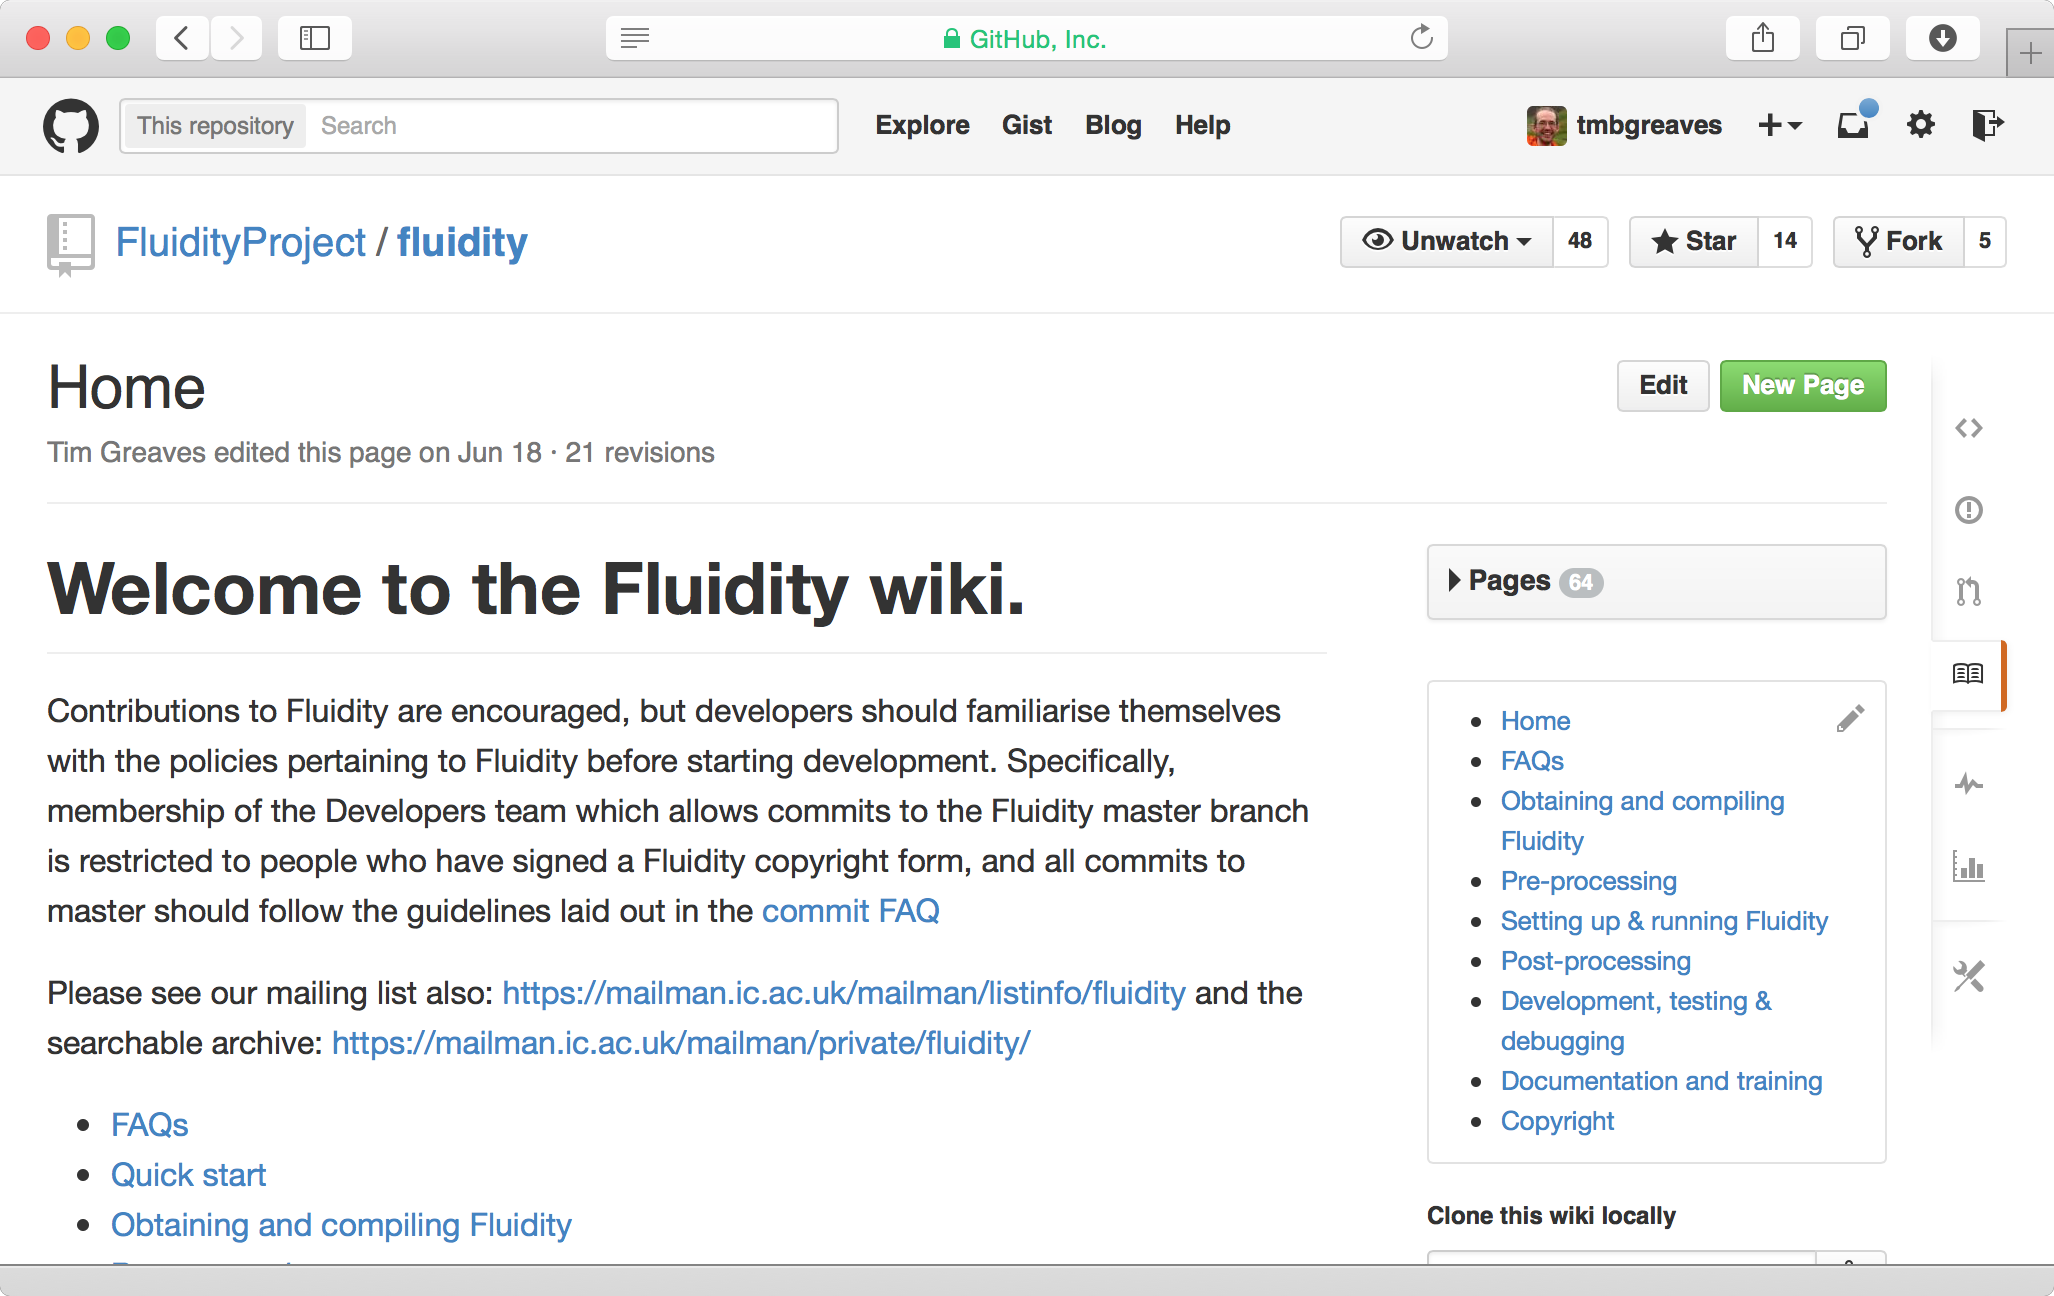
\includegraphics[width=0.9\textwidth]{images/github-wiki.png}
\end{center}
\end{frame}

\begin{frame}
\begin{center}
http://buildbot-ocean.ese.ic.ac.uk:8080/waterfall

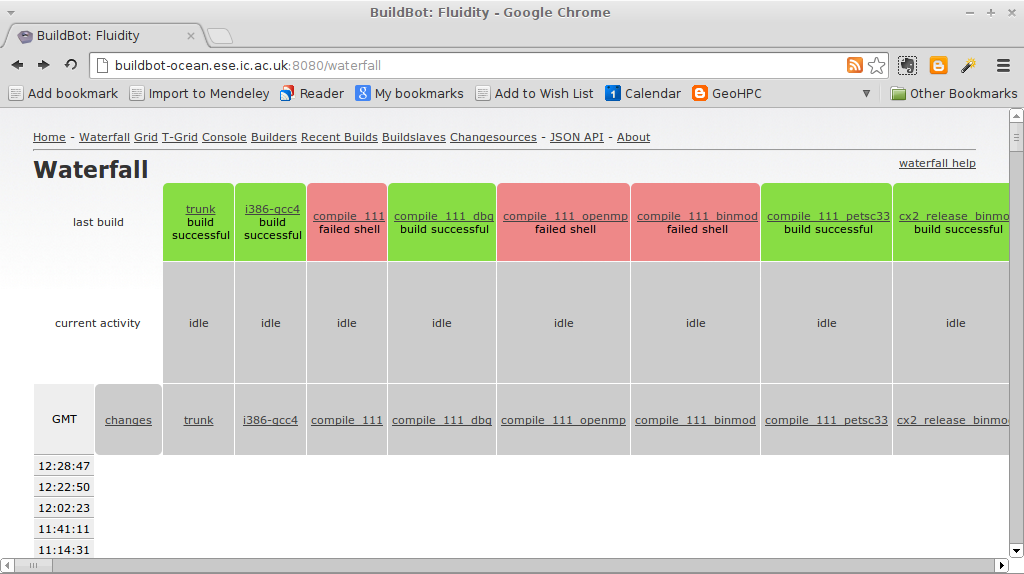
\includegraphics[width=0.9\textwidth]{images/buildbot.png}
\end{center}
\end{frame}

\section{Configuring and building}
\begin{frame}[fragile]
        \frametitle{Configure}
Set up compile-time options, such as:
\begin{itemize}
    \item External non-LGPL libraries
    \item Non-standard libray locations
    \item Compiler flags
    \item Debugging
\end{itemize}
\lstset{language=bash}
\begin{lstlisting}[language=bash,basicstyle=\ttfamily]
cd [fluidity directory]
./configure --enable-2d-adaptivity
\end{lstlisting}
\end{frame}

\begin{frame}[fragile]
        \frametitle{Building}
\lstset{language=bash}
Before building Fluidity, clean your source code:
\begin{lstlisting}[language=bash,basicstyle=\ttfamily]
make clean
\end{lstlisting}
Now make the main code:
\begin{lstlisting}[language=bash,basicstyle=\ttfamily]
make -j 4
\end{lstlisting}
And build the Fluidity tool suite:
\begin{lstlisting}[language=bash,basicstyle=\ttfamily]
make fltools
\end{lstlisting}



\end{frame}

\begin{frame}[fragile]
    \frametitle{Python}
\lstset{language=bash}
Fluidity contains several Python packages that are required for it to run.  
Where you have not installed Fluidity system-wide, the Fluidity python
directory must be added to the existing environment variable PYTHONPATH.

From the fluidity/ directory, run:
\begin{lstlisting}[language=bash,basicstyle=\ttfamily\footnotesize]
export PYTHONPATH=$PYTHONPATH:$PWD/python
\end{lstlisting}
This can be checked by using the echo command.
\begin{lstlisting}[language=bash,basicstyle=\ttfamily\footnotesize]
echo $PYTHONPATH
\end{lstlisting}
\end{frame}

\section{Testing}
\begin{frame}[fragile]
        \frametitle{Tests}
\lstset{language=bash}

To check that all the verification tests run and pass with 
your Fluidity build, you can issue the following commands:

\begin{lstlisting}[language=bash,basicstyle=\ttfamily]
make unittest
make test
make mediumtest
\end{lstlisting}
\end{frame}

\begin{frame}[fragile]
        \frametitle{Installing}
\lstset{language=bash}
Installing Fluidity enables access for all other users of your computer; this
may require 'sudo' or other administrative access.
\begin{lstlisting}[language=bash,basicstyle=\ttfamily]
make install
make install-diamond
make install-user-schemata
\end{lstlisting}
\end{frame}

\begin{frame}
    \frametitle{Running Fluidity}
From source:    
\\ \texttt{<fluidity-clone>/bin/fluidity -v2 -l [filename].flml}
\\ [0.5cm]
From binary:    
\\ \texttt{fluidity -v2 -l [filename].flml}
\end{frame}

\begin{frame}[fragile]
        \frametitle{Updating}
\lstset{language=bash}
If you want to update your local clone of the Fluidity repository to the newest
commit, run:

\begin{lstlisting}[language=bash,basicstyle=\ttfamily]
git pull
\end{lstlisting}

from within the local clone.

\end{frame}

\end{document}

